\chapter{Verzamelingen}\label{ch:verzamelingen}
%\begin{remark}
%De hierop volgende onderdelen in sectie \ref{sec:venn} tot aan het begin van sectie \ref{sec:operator} zijn een grotendeels een herhaling van het materiaal beschikbaar voor de cursus `Analytical Skills' (TICT-V1ASK-17). Ze zijn hier opgenomen als herhaling van het lesmateriaal.
%\end{remark}
In de meest uiteenlopende omstandigheden kan het handig zijn om een stel objecten, elementen, of wat dan ook, samen een naam te geven. Het resultaat noemen we dan een \textit{verzameling}. Zo'n verzameling bestaat alleen maar bij de gratie van de elementen die erin zitten.

Het fundamentele verband tussen een verzameling en objecten is dat van elk object vast ligt of het behoort tot die verzameling of niet. Synoniemen voor ``behoren tot'' zijn ``lid zijn van'' en ``element zijn van''. Deze zullen door elkaar worden gebruikt, maar betekenen hetzelfde.

We gebruiken het \textit{esti-teken} $\in$ als afkorting voor ``is element van'', zoals in $x\in A$, waarmee we dus uitdrukken dat ``$x$ een element is van (verzameling) $A$''. Als iets geen element is van een verzameling, dan gebruiken we $\not\in$, bijv. $y\not\in A$ om uit te drukken dat $y$ niet in de verzameling $A$ zit.

Heeft een verzameling slechts eindig veel elementen, dan kunnen we die elementen allemaal \textit{opsommen}, en daardoor de verzameling defini\"eren. De standaardnotatie die we daarvoor gebruiken is het achter elkaar opschrijven van de elementen, gescheiden door komma's, en het geheel afsluiten met accolades. Bijvoorbeeld
$$V=\{3,4,9,1\}$$
$$W=\{\text{maandag},\text{dinsdag},\text{woensdag},\text{donderdag},\text{vrijdag},\text{zaterdag},\text{zondag}\}$$
Merk op dat het er niet toe doet in welke volgorde de elementen tussen de accolades staan. Ook mogen elementen herhaald worden:
$$\{3, 4,9,1\}=\{1,3,4,9\}=\{3,4,9,3,1\}$$
Soms gebruiken we ook een suggestieve notatie zoals in
$$A=\{1,2,\ldots,10\}\qquad B=\{3,4,5,\ldots\}$$
Een waarschuwing is hier wel op zijn plaats: in zijn algemeenheid is het niet precies duidelijk wat `\ldots' betekent, en is het aan te raden dit alleen te gebruiken als iedereen er dezelfde betekenis aan hecht. Wat zou bijvoorbeeld 
$$\{1,2,4,8,16,\ldots\}$$
betekenen? De meeste mensen zullen dit rijtje wel verder kunnen bedenken op de manier waarin elk getal door verdubbelen uit het vorige verkregen is, maar andere interpretaties zijn ook mogelijk. Voor grotere verzamelingen, waarbij de neiging bestaat om puntjes te gebruiken hebben we behoefte aan een andere notatie.

Om te beginnen, spreken we voor een aantal veel gebruikte verzamelingen af dat we ze altijd met een vast teken zullen introduceren. Zo kennen we de standaard notaties
\begin{center}
    \begin{tabular}{ll}
    $\varnothing$ & voor de \textit{lege verzameling}, zonder elementen.\\
    $\mathbb{N}$ & voor de verzameling van alle \textit{natuurlijke getallen},\\
    $\mathbb{Z}$ & voor de verzameling van alle \textit{gehele getallen},\\
    $\mathbb{Q}$ & voor de verzameling van alle \textit{rationele getallen},\\
    $\mathbb{R}$ & voor de verzameling van alle \textit{re\"ele getallen},\\
    $\mathbb{C}$ & voor de verzameling van alle \textit{complexe getallen}.
    \end{tabular}
\end{center}
De keuze van de letters $\mathbb{N}, \mathbb{R}$ en $\mathbb{C}$ spreken voor zich, de keuze van de letter $\mathbb{Q}$ is ontleend aan `quoti\"ent', terwijl de keuze van de letter $\mathbb{Z}$ afkomstig is van het Duitse woord `Zahlen' (`getallen' of `tellen').

Bij $\mathbb{N}$ en $\mathbb{Z}$ zouden we voor een redelijk ervaren lezer ook de puntjes-notatie ($\mathbb{N}=\{0,1,2,3,4,\ldots\}$ en $\mathbb{Z}=\{\ldots,-2,-1,0,1,2,\ldots\}$) kunnen gebruiken. Voor $\mathbb{Q}, \mathbb{R}$ en $\mathbb{C}$ kan dat niet. $\mathbb{Q}$ is de verzameling van quotienten, ofwel alle getallen die te schrijven zijn als een deling $\frac{n}{m}$ voor getallen $n,m\in\mathbb{Z}$, dus bijvoorbeeld $\frac{1}{2}$, maar ook $\frac{-1}{1} (=-1)$ of $\frac{-1000}{-20}$, etc.

De verzameling $\mathbb{R}$ is vervolgens een uitbreiding met alle getallen die te schrijven zijn als een of ander komma-getal, bijvoorbeeld $\sqrt{2}$, %\footnote{Zie ook het bewijs dat $\sqrt{2}$ geen rationeel getal is in opgave \ref{ex:sqrt:2} op pagina \pageref{ex:sqrt:2}.}, 
of $\pi$. De verzameling $\mathbb{C}$ van complexe getallen\footnote{Volledig begrip van de verzameling $\mathbb{R}$, maar vooral $\mathbb{C}$, ligt buiten de scope van deze cursus.}, tenslotte, is de aanvulling met het imaginaire getal $i$ waarvoor geldt dat $i^2=-1$.

Vaak stoppen we objecten in een verzameling omdat ze alle een specifieke eigenschap hebben die ons interesseert. Zo schrijven we bijvoorbeeld\footnote{Lees $\{x\in\mathbb{Z}\;|\;1\leq x\leq 10\}$ als `de verzameling ($\{\ldots\}$) van gehele getallen $x$ ($x\in\mathbb{Z}$), waarvoor geldt dat ($|$) $x$ tussen 1 en 10 is.}
$$A=\{x\in\mathbb{Z}\;|\;1\leq x\land x\leq 10\}$$
om aan te geven dat $A$ bestaat uit alle gehele getallen tussen (inclusief) $1$ en $10$. Dit is dus dezelfde verzameling als
$$A=\{1,2,3,\ldots,10\},$$
maar we behoeven niet te raden wat de puntjes betekenen, en we hoeven ook niet alle elementen op te sommen. In zijn algemeenheid kunnen we altijd eigenschappen gebruiken om een verzameling te defini\"eren. 

Normaliter defini\"eren we verzamelingen binnen een bepaalde \textit{context}; het \textit{universum} $U$. Als de verzameling $U$ steeds dezelfde is, en het is duidelijk wat het universum is (bijvoorbeeld $\mathbb{Z}$ in het voorgaande voorbeeld), dan kunnen we de verzameling $A$ ook opschrijven als
$$A=\{x\;|\;1\leq x\leq 10\}.$$

Merk op dat de lege verzameling zodanig ook te defini\"eren is als
$$\varnothing=\{x\;|\;\bot\}.$$
Hierin hebben we het universum weggelaten omdat dit er toch niet toe doet (er is geen enkel universum waarvoor de eigenschap $\bot$ elementen levert aan de lege verzameling). 

Een verzameling $A$ heet een \textit{deelverzameling} van een verzameling $B$ als elk element in $A$ ook een element is van $B$. We gebruiken hiervoor de notatie $A\subseteq B$, en soms ook wel $B\supseteq A$. Dus:
$$A\subseteq B\text{ betekent dat voor alle elementen $x$, als $x\in A$ dan $x\in B$.}$$
De relatie $\subseteq$ heet ook wel \textit{inclusie}. Een verzameling $A$ heet een \textit{echte deelverzameling} van een verzameling $B$ als $A\subseteq B$ \'en er een element van $B$ is dat niet een element van $A$ is. Hiervoor wordt wel de notatie $A\subset B$ gebruikt, en soms ook wel $B\supset A$. Voor de eerder genoemde veel gebruikte verzamelingen kunnen we nu zien dat
$$\mathbb{N}\subset\mathbb{Z}\subset\mathbb{Q}\subset\mathbb{R}\subset\mathbb{C},$$
dat wil zeggen, alle natuurlijke getallen zijn ook gehele getallen, etc.

Twee verzamelingen $A$ en $B$ zijn \textit{gelijk} (notatie $A=B$) als ze dezelfde elementen bevatten, dus precies dan als $A\subseteq B$ en $B\subseteq A$.
$$A=B\text{ betekent dat voor alle elementen $x$, $x\in A$ dan en slechts dan als $x\in B$.}$$

\begin{aside}[Russell's Paradox]\label{as:russel:paradox}\mbox{}\\
Een belangrijk voorbeeld van problemen die kunnen ontstaan als er te weinig duidelijkheid wordt gegeven in de definitie van verzamelingen is de \emph{Russell's Paradox}, reeds eerder aangehaald in Terzijde \ref{as:frege} op pagina \pageref{as:frege}.

De paradox gaat ongeveer als volgt. In de verzamelingenleer is het mogelijk om verzamelingen van verzamelingen te defini\"eren, bijvoorbeeld, de verzameling van AI-klassen $K = \{AI\text{-}V1A, AI\text{-}V1B, \ldots\}$, waarvan de elementen zelf, duidelijk, ook weer verzamelingen zijn (namelijk van de studenten waaruit die klas is opgemaakt). Dat wil zeggen dat $K$ is opgebouwd uit de verzameling van verzamelingen eerstejaars AI-studenten. Merk op dat de verzameling $K$ geen onderdeel is van zichzelf, immers $K$ is geen verzameling van eerstejaars AI-studenten. 

Echter is er een verzameling te defini\"eren, $\mathbf{R}$ de Russellverzameling, die opgebouwd is uit alle verzamelingen die \emph{niet} zichzelf bevatten; ofwel $\mathbf{R} = \{V\;|\;V\not\in V\}$. Deze verzameling is niet leeg (immers $K$ bevat niet zichzelf, dus $K\in\mathbf{R}$. Maar zit $\mathbf{R}\in\mathbf{R}$? Dat wil zeggen, bevat $\mathbf{R}$ zichzelf?

Stel dat $\mathbf{R}\in\mathbf{R}$, als dat zo is, dan moet ze ook voldoen aan de definitie van $\mathbf{R}$, oftewel $\mathbf{R}\not\in\mathbf{R}$. Maar dat is in tegenspraak met onze aanname.

Stel dat $\mathbf{R}\not\in\mathbf{R}$, maar als dat zo is, dan zou $\mathbf{R}\in\mathbf{R}$, want $\mathbf{R}$ is immers de verzameling van alle verzamelingen die niet in zichzelf zitten.

Beide aannames leiden tot een tegenspraak en het is derhalve onmogelijk om te bepalen of $\mathbf{R}\in\mathbf{R}$ of $\mathbf{R}\not\in\mathbf{R}$. 

Zoals eerder vermeld, heeft deze paradox de wereld van de wiskunde grondig op zijn kop gezet. Het heeft enige jaren en vele kopzorgen geduurd alvoor Russell bedacht had hoe dit probleem op te lossen was, zonder een geheel nieuwe theoretisch basis voor de wiskunde te bedenken. De oplossing door middel van typetheorie valt echter buiten de scope van deze cursus om hier te behandelen.
\end{aside}

\section{Venn-diagrammen}\label{sec:venn}
Het is eenvoudiger om over dingen na te denken als je er een plaatje van kan maken. Visuele stimuli kunnen je brein helpen om problemen op te lossen, wat de reden is waarom, als je aan een wiskundig probleem werkt, het vaak helpt om eerst een plaatje te tekenen. Het maken van een plaatje alleen voorkomt dat je zit te dagdromen en dat je gedachten, tijdens het oplossen van het probleem, wendingen nemen die je niet helpen bij het nadenken. De Engelsman John Venn (1834 -- 1923) introduceerde een systematisch manier om schetsen te maken als visueel hulpmiddel voor het nadenken over verzamelingen (en logica); we noemen dergelijke diagrammen \textit{Venn-diagrammen}.

\begin{figure}[ht]
    \centering
    \begin{tikzpicture}[scale=.6]
    \draw[thick,fill=gray!20] (0,0) rectangle (7,5);
    \node at (6.5,4.5) {$U$};
    \draw[fill=hublue!20] (2.5,2.5) circle (1.5cm);
    \draw[fill=hublue!40] (4.5,2.5) circle (1.5cm);
    \begin{scope}
      \clip (4.5,2.5) circle (1.49cm);
      \draw[fill=hured!20] (2.5,2.5) circle (1.5cm);
    \end{scope}
    \node at (1.75,3.5) {$A$};
    \node at (5.25,3.5) {$B$};
    \end{tikzpicture}\hspace{1cm} 
    \begin{tikzpicture}[scale=.6]
    \draw[thick, fill=gray!20] (0,0) rectangle (7,5);
    \node at (6.5,4.5) {$U$};
    \draw[fill=hublue!20] (1.75,2.5) circle (1.5cm);
    \draw[fill=hublue!40] (5.25,2.5) circle (1.5cm);
    \node at (1,3.5) {$A$};
    \node at (6,3.5) {$B$};
    \end{tikzpicture}
    \caption{Overlappende (links) en disjoint (rechts) verzamelingen.}
    \label{fig:disjunct}
\end{figure}

Hierboven zijn twee Venn-diagrammen getekend voor de verzamelingen $A$ en $B$. We stellen ons voor dat $A$ bestaat uit alle punten in de cirkel $A$\footnote{Merk op dat in veel gevallen, Venn-diagrammen \textit{abstraheren} van de specifieke inhoud van de getekende verzamelingen; dat wil zeggen, de objecten/individuen die in een verzameling worden meestal niet getekend om het plaatje overzichtelijker te maken.} en we maken dezelfde aanname over $B$. De grote rechthoek waar beide verzamelingen inzitten representeert het universum $U$. Het linker diagram toont dat $A$ en $B$ een \textit{overlap} hebben, terwijl het rechter toont dat $A$ en $B$ \textit{disjunct} zijn. (Over het algemeen worden cirkels of ovalen gebruikt om verzamelingen aan te duiden, maar andere vormen, zoals rechthoeken, mogen ook worden gebruikt. Tevens is het gebruik van kleur niet noodzakelijk, maar het maakt de diagrammen wel mooier).

Merk op dat, omdat we abstraheren van de specifieke individuen (d.w.z., we tekenen de elementen in de verzamelingen niet), het nog steeds zo kan zijn dat de overlap tussen $A$ en $B$ in de linkerkant van figuur \ref{fig:disjunct} leeg is. Alleen als we alle elementen zouden tekenen, en er daadwerkelijk elementen in het rode gebied zouden zitten, kunnen we stellen dat $A$ en $B$ een \textit{niet-lege} overlap hebben.

\section{Operatoren op verzamelingen}\label{sec:operator}
Bij twee verzamelingen $A$ en $B$ die niet gelijk zijn, kunnen we een hele serie nieuwe verzamelingen defini\"eren. Dat gaan we nu doen.

Met $A\cap B$ duiden we de \textit{doorsnede} van $A$ en $B$ aan: de verzameling die bestaat uit alle objecten die zowel in $A$ als in $B$ zitten, oftewel
$$A\cap B=\{x\;|\; x\in A\land x\in B\},$$
ook te schrijven als
$$A\cap B=\{x\in A\;|\; x\in B\},$$
en ook als
$$A\cap B=\{x\in B\;|\; x\in A\}.$$

Een belangrijke equivalentie die direct volgt uit deze definitie is
$$x\in A\cap B\quad\Leftrightarrow\quad x\in A\land x\in B.$$

Twee verzamelingen heten \textit{disjunct} als hun doorsnede leeg is.
\begin{figure}[ht]
    \centering
    \begin{tikzpicture}[scale=.6]
    \draw[thick,fill=gray!20] (0,0) rectangle (7,5);
    \node at (6.5,4.5) {$U$};
    \draw[fill=hublue!20] (2.5,2.5) circle (1.5cm);
    \draw[fill=hublue!40] (4.5,2.5) circle (1.5cm);
    \begin{scope}
      \clip (4.5,2.5) circle (1.49cm);
      \draw[fill=hured!60] (2.5,2.5) circle (1.5cm);
    \end{scope}
    \node at (1.75,3.5) {$A$};
    \node at (5.25,3.5) {$B$};
    \node at (3.5, 4.25) {\color{hured}$A\cap B$};
    \end{tikzpicture}\hspace{1cm} 
    \begin{tikzpicture}[scale=.6]
    \draw[thick,fill=gray!20] (0,0) rectangle (7,5);
    \node at (6.5,4.5) {$U$};
    \draw[fill=hured!60] (2.5,2.5) circle (1.5cm);
    \draw[fill=hured!60] (4.5,2.5) circle (1.5cm);
    \begin{scope}
      \clip (4.5,2.5) circle (1.49cm);
      \draw[fill=hured!60] (2.5,2.5) circle (1.5cm);
    \end{scope}
    \node at (1.75,3.5) {$A$};
    \node at (5.25,3.5) {$B$};
    \node at (3.5, 4.25) {\color{hured}$A\cup B$};
    \end{tikzpicture}
    \caption{De \textit{doorsnede} van $A$ en $B$: $A\cap B$ (links) en de \textit{vereniging} van $A$ en $B$: $A\cup B$ (rechts).}
    \label{fig:intersect:union}
\end{figure}

Met $A\cup B$ duiden we de \textit{vereniging} van $A$ en $B$ aan: de verzameling die bestaat uit alle objecten van $A$ en alle objecten van $B$, oftewel
$$A\cup B=\{x\;|\; x\in A\lor x\in B\}.$$
Een belangrijke equivalentie die direct volgt uit deze definitie is
$$x\in A\cup B\quad\Leftrightarrow\quad x\in A\lor x\in B.$$

Met $A-B$, het \textit{verschil} van $A$ en $B$, bedoelen we de verzameling bestaande uit alle objecten die wel tot $A$ behoren, maar niet tot $B$, oftewel
$$A-B=\{x\in A\;|\;x\not\in B\}.$$
Een belangrijke equivalentie die direct volgt uit deze definitie is
$$x\in A-B\quad\Leftrightarrow\quad x\in A\land x\not\in B.$$

De verzameling $(A\cup B)-(A\cap B)$ staat bekend als \textit{symmetrisch verschil} van $A$ en $B$. Deze is gelijk aan $(A-B)\cup(B-A)$ zoals we later nog zullen zien. Hiervoor wordt ook wel de notatie $A\;\Delta\;B$ gebruikt.
\begin{figure}[ht]
    \centering
    \begin{tikzpicture}[scale=.6]
    \draw[thick,fill=gray!20] (0,0) rectangle (7,5);
    \node at (6.5,4.5) {$U$};
    \draw[fill=hured!60] (2.5,2.5) circle (1.5cm);
    \draw[fill=hublue!40] (4.5,2.5) circle (1.5cm);
    \begin{scope}
      \clip (4.5,2.5) circle (1.49cm);
      \draw[fill=hublue!40] (2.5,2.5) circle (1.5cm);
    \end{scope}
    \node at (1.75,3.5) {$A$};
    \node at (5.25,3.5) {$B$};
    \node at (3.5, 4.25) {\color{hured}$A-B$};
    \end{tikzpicture}\hspace{1cm} 
    \begin{tikzpicture}[scale=.6]
    \draw[thick,fill=gray!20] (0,0) rectangle (7,5);
    \node at (6.5,4.5) {$U$};
    \draw[fill=hured!60] (2.5,2.5) circle (1.5cm);
    \draw[fill=hured!60] (4.5,2.5) circle (1.5cm);
    \begin{scope}
      \clip (4.5,2.5) circle (1.49cm);
      \draw[fill=hublue!40] (2.5,2.5) circle (1.5cm);
    \end{scope}
    \node at (1.75,3.5) {$A$};
    \node at (5.25,3.5) {$B$};
    \node at (3.5, 4.25) {\color{hured}$A\;\Delta\; B$};
    \end{tikzpicture}
    \caption{Het \textit{verschil} van $A$ en $B$: $A-B$ (links) en het \textit{symmetrische verschil} van $A$ en $B$: $A\;\Delta\; B$ (rechts).}
    \label{fig:diff:symdif}
\end{figure} 

Zoals gezegd komt het vaak voor dat we het uitsluitend willen hebben over objecten in een vast \textit{universum} $U$. Dat houdt tevens in dat alle verzamelingen waarover we dan kunnen spreken deelverzamelingen zijn van $U$. Is $U$ het universum, dan heet $U-A$ het \textit{complement} van $A$, ook wel korter genoteerd als $A^c$:
$$A^c=\{x\;|\;x\not\in A\}.$$
\begin{figure}[ht]
    \centering
    \begin{tikzpicture}[scale=.6]
    \draw[thick,fill=hured!60] (0,0) rectangle (7,5);
    \node at (6.5,4.5) {$U$};
    \draw[fill=hublue!20] (2.5,2.5) circle (1.5cm);
    \node at (1.75,3.5) {$A$};
    \node at (0.5, 4.5) {\color{hured}$A^c$};
    \end{tikzpicture}
    \caption{Het \textit{complement} van verzameling $A$: $A^c$.}
    \label{fig:complement}
\end{figure}

Zoals al deels te begrijpen valt uit de definities van de operatoren hierboven, is er een sterke analogie tussen propositielogica en verzamelingenleer. Deze analogie is nog sterker in een uitbreiding van de propositielogica: de predikaatlogica welke later in deze cursus behandelt zal worden (zie hoofdstuk \ref{ch:predicaten}). 

Voor de operatoren die hierboven beschreven zijn, zijn ook rekenregels te defini\"eren, analoog aan hoe er, bijvoorbeeld in de wiskunde, met de $+$- en $\times$-operatoren wordt omgegaan.
\begin{theorem}\mbox{}\\
Voor alle verzamelingen $A$, $B$ en $C$ gelden de volgende regels:
\begin{enumerate}
    \item $A\cup\varnothing = A$
    \item $A\cap\varnothing = \varnothing$
    \item $A\cup B=B\cup A$
    \item $A\cap B=B\cap A$
    \item $(A\cup B)\cup C=A\cup (B\cup C)$
    \item $(A\cap B)\cap C=A\cap(B\cap C)$
    \item $(A\cup B)\cap C=(A\cap C)\cup(B\cap C)$
    \item $(A\cap B)\cup C=(A\cup C)\cap(B\cup C)$
\end{enumerate}\label{th:regels}
\end{theorem}
Hierin drukt regel 1 uit dat $\varnothing$ een \textit{neutraal element} is met betrekking tot de vereniging. Regels 3 en 4 geven aan dat vereniging en doorsnede \textit{commutatief} zijn. Regels 5 en 6 geven aan dat vereniging en doorsnede \textit{associatief} zijn. Regel 7 geeft aan dat doorsnede \textit{distribueert over} vereniging en regel 8 geeft aan dat vereniging distribueert over doorsnede.

Om deze stelling te kunnen bewijzen zullen we een aantal keren bewijs geven dat twee deelverzamelingen $V$ en $W$ gelijk aan elkaar zijn. Per definitie betekent dat dat elk element van $V$ in $W$ moet zitten en omgekeerd. Dit zouden we volgens de volgende twee `halve bewijzen' kunnen doen:
\begin{itemize}
    \item kies een willekeurig element in $V$ en bewijs dat die in $W$ zit;
    \item kies een willekeurig element in $W$ en bewijs dat die in $V$ zit.
\end{itemize}
Vaak kunnen we zo'n bewijs echter korter opschrijven:
$$x\in V\Leftrightarrow\ldots\Leftrightarrow\ldots\ldots\ldots\Leftrightarrow x\in W$$
dan hebben we daarmee het eerste halve bewijs gegeven door deze reeks van links naar rechts te lezen, en hebben we het tweede halve bewijs gegeven door deze reeks van rechts naar links te lezen. We geven enkele voorbeelden van dergelijke bewijzen. Steeds schrijven we stap voor stap de motivatie voor de geldigheid tussen haakjes, er achter, in dezelfde stijl zoals we dat al eerder deden. Equivalenties in deze redeneringen noteren we met $\Leftrightarrow$; deze notatie geeft de twee richtingen aan waarin we het bewijs kunnen lezen. We beginnen met het bewijs van regel 1 van Stelling \ref{th:regels}.
\begin{center}
    \begin{tabular}{ccll}
        $x\in A\cup\varnothing$ & $\Leftrightarrow$ & $x\in A\lor x\in\varnothing$ & (definitie $\cup$) \\
        & $\Leftrightarrow$ & $x\in A\lor\bot$ & (definitie $\varnothing$)\\
        & $\Leftrightarrow$ & $x\in A$ & (St \ref{th:equiv}: 1)
    \end{tabular}
\end{center}
Vanwege $x\in A\cup\varnothing\Leftrightarrow x\in A$ geldt nu $A\cup\varnothing=A$ en is regel 1 van Stelling \ref{th:regels} bewezen.

We bewijzen nu regel 8 van Stelling \ref{th:regels}.
\begin{center}
    \begin{tabular}{ccll}
        $x\in(A\cap B)\cup C$ & $\Leftrightarrow$ & $x\in(A\cap B)\lor x\in C$ & (definitie $\cup$)\\
        & $\Leftrightarrow$ & $(x\in A\land x\in B)\lor x\in C$ & (definitie $\cap$)\\
        & $\Leftrightarrow$ & $(x\in A\lor x\in C)\land(x\in B\lor x\in C)$ & (St \ref{th:equiv}: 12)\\
        & $\Leftrightarrow$ & $(x\in A\cup C)\land(x\in B\lor x\in C)$ & (definitie $\cup$)\\
        & $\Leftrightarrow$ & $(x\in A\cup C)\land(x\in B\cup C)$ & (definitie $\cup$)\\
        & $\Leftrightarrow$ & $x\in(A\cup C)\cap(B\cup C)$ & (definitie $\cap$)
    \end{tabular}
\end{center}
Vanwege $x\in (A\cap B)\cup C\Leftrightarrow x\in(A\cup C)\cap(B\cup C)$ geldt nu $(A\cap B)\cup C=(A\cup C)\cap(B\cup C)$, en is dus ook regel 8 van Stelling \ref{th:regels} bewezen. De bewijzen van de overige regels van Stelling \ref{th:regels} gaan geheel analoog. We zien ook dat het geen toeval is dat dezelfde regels die we in de propositierekening tegenkwamen voor $\lor$ en $\land$ hier precies zo gelden voor $\cup$ en $\cap$: bij het toepassen van de definities van $\cup$ en $\cap$ vertaalt elk $\cup$-symbool naar $\lor$, elk $\cap$-symbool naar $\land$ en $\varnothing$ naar $\bot$, waarna de bijbehorende regel uit de propositierekening toegepast wordt, en vervolgens nog een aantal keren de definities van $\cup$ en $\cap$ tot het gewenste resultaat is bereikt.

Aan de ene kant is deze analogie handig, aan de andere kant is een waarschuwing hier ook op zijn plaats: $\cup$ en $\cap$ zijn operatoren die altijd op verzamelingen werken, en $\lor$ en $\land$ zijn operatoren die altijd op proposities / beweringen werken. Haal ze dus niet door elkaar.

\begin{theorem}
Voor alle verzamelingen $A$, $B$ en $C$ gelden de volgende regels
\begin{enumerate}
    \item $\varnothing\subseteq A$
    \item $A\subseteq(A\cup B)$
    \item $(A\cap B)\subseteq A$
    \item als $A\subseteq B$, dan $(A\cup C)\subseteq(B\cup C)$
    \item als $A\subseteq B$, dan $(A\cap C)\subseteq(B\cap C)$
    \item als $A\subseteq C$ en $B\subseteq C$, dan $(A\cup B)\subseteq C$
    \item als $A\subseteq B$ en $A\subseteq C$, dan $A\subseteq(B\cap C)$
    \item als $A\subseteq B$ en $B\subseteq C$, dan $A\subseteq C$
\end{enumerate}\label{th:inclusie}
\end{theorem}
Regel 8 drukt uit dat inclusie \textit{transitief} is.

Het bewijs van een bewering $V\subseteq W$ gaat vrijwel altijd als volgt: neem een willekeurig element $x\in V$ en bewijs dat $x\in W$. Als voorbeeld bewijzen we $\varnothing\subseteq A$. Neem een willekeurig element $x\in\varnothing$. Zo'n element bestaat helemaal niet: de aanname is $\bot$. Uit $\bot$ kunnen we alles concluderen, in het bijzonder dat $x\in A$. Hiermee is bewezen dat $\varnothing\subseteq A$, oftewel regel 1 van Stelling \ref{th:inclusie}.

Nu gaan we regel 4 van Stelling \ref{th:inclusie} bewijzen. Volgens het deductieprincipe nemen we aan dat $A\subseteq B$, en moeten we op grond daarvan bewijzen dat $(A\cup C)\subseteq(B\cup C)$. Kies daartoe een willekeurig element $x\in A\cup C$, per definitie geldt dan $x\in A\lor x\in C$. Om deze disjunctie te gebruiken hebben we een gevalsonderscheiding nodig. We schrijven het bewijs nog maar eens in detail in stappen op:
\begin{proof}\mbox{}\\
\begin{tabular}{lll}
(1) & $x\in A\cup C$ & (aanname) \\
(2) & $x\in A\lor x\in C$ & (1, definitie $\cup$)\\
(3) & $x\in A\vdash x\in B\cup C$\\
& bewijs van 3:\\
& \multicolumn{2}{l}{\begin{tabular}{lll}
        (3.1) & $x\in A$ & (veronderstelling)\\
        (3.2) & $x\in B$ & (3.1, aanname $A\subseteq B$)\\
        (3.3) & $x\in B\lor x\in C$ & (3.2, introductie $\lor$)\\
        (3.4) & $x\in B\cup C$ & (3.3, definitie $\cup$)
    \end{tabular}}\\
(4) & $x\in C\vdash x\in B\cup C$\\
& bewijs van 4:\\
& \multicolumn{2}{l}{\begin{tabular}{lll}
    (4.1) & $x\in C$ & (veronderstelling)\\
    (4.2) & $x\in B\lor x\in C$ & (4.1, introductie $\lor$)\\
    (4.3) & $x\in B\cup C$ & (4.2, definitie $\cup$)
\end{tabular}}\\
(5) & $x\in B\cup C$ & (2, 3, 4, gevalsonderscheiding)
\end{tabular}\\
Hiermee hebben we bewezen dat $x\in B\cup C$ voor elk willekeurig element $x\in A\cup C$, oftewel $(A\cup C)\subseteq(B\cup C)$.
\end{proof}
Daarmee is regel 4 van Stelling \ref{th:inclusie} bewezen. Opvallend is de constructie die gebruikt is in stap (3) en (4) van het bewijs. Dit is een gevalsonderscheiding waarbij, vanuit het gegeven dat $x\in A\lor x\in C$ (conclusie van (2)) bepaald wordt dat er twee mogelijke gevallen zijn: $x\in A$ (stap (3)) of $x\in C$ (stap (4)). Als kan worden aangetoond dat voor beide gevallen dezelfde conclusie getrokken kan worden, dan kunnen we die conclusie in zijn algemeen trekken. 

De andere stap die verdere uitleg behoeft is stap (3.3) (en evenzo (4.2)): vanuit $x\in B$ concluderen we dat $x\in B\lor x\in C$. Deze stap heet `verzwakking' (of $\lor$-introductie), aangezien het gegeven wordt verzwakt met 'overbodige' informatie. Immers, als we al weten dat $x\in B$, dan weten we ook dat $x\in B\lor x\in C$ (de linkerzijde van de $\lor$ is immers waar, en daarom is de gehele propositie ook waar). %Oplettende lezers bemerken dat deze regels al waren ge\"introduceerd in sectie \ref{sec:nat:deduc}.

In woorden zouden we ditzelfde bewijs ook iets slordiger zo op kunnen schrijven:
\begin{proof}
We weten $x\in A\lor x\in C$ en maken nu een gevalsonderscheiding tussen $x\in A$ en $x\in C$. Als $x\in A$ dan $x\in A\subseteq B\subseteq B\cup C$. Als $x\in C$ dan $x\in C\subseteq B\cup C$. In beide gevallen hebben we $x\in B\cup C$, dus geldt $x\in B\cup C$.
\end{proof}
De slordigheid in dit laatste bewijs zit hem in het weglaten van details als nummertjes en namen van regels; maar afgezien daarvan is het precies hetzelfde, en is elk detail weer desgewenst in te vullen. Als daaraan voldaan is, zullen we ook dit soort `slordige' bewijzen toestaan. Met nadruk wijzen we erop dat dit geen water in de wijn doet op het gebied van precisie, en zeker niet gebruikt kan worden om ontbrekende stukken van een redenering onder het tapijt te vegen. Het vinden van een bewijs blijft even moeilijk en de gestelde eisen aan een redenering blijven dezelfde, we staan alleen een beknoptere en misschien begrijpelijkere notatie van het eindresultaat toe.

Het bewijs van de overige regels van Stelling \ref{th:inclusie} laten we aan de lezer over.

We geven nu een aantal gelijkheden met betrekking tot het \textit{complement} van verzamelingen.
\begin{theorem}
In een vast universum $U$ gelden de volgende regels voor verzamelingen $A$ en $B$
\begin{enumerate}
    \item $\varnothing^c=U$
    \item $U^c=\varnothing$
    \item $(A^c)^c=A$
    \item $(A\cup B)^c=A^c\cap B^c$
    \item $(A\cap B)^c=A^c\cup B^c$
    \item als $A\subseteq B$, dan $B^c\subseteq A^c$
\end{enumerate}\label{th:compl}
\end{theorem}
We zien dat bij Stelling \ref{th:regels} genoemde analogie tussen operatoren voor proposities en operatoren voor verzamelingen zich nog verder uitbreidt: het complement vertaalt naar $\neg$ en het universum $U$ naar $\top$. De basisregels zijn
$$x\in\varnothing\Leftrightarrow\bot,\qquad x\in U\Leftrightarrow\top,\qquad x\in A^c\Leftrightarrow\neg(x\in A),$$
$$x\in A\cup B\Leftrightarrow(x\in A\lor x\in B),\qquad x\in A\cap B\Leftrightarrow(x\in A\land x\in B).$$
Samen met de propositierekening kunnen we hiermee rechtstreeks de eerste vijf regels van Stelling \ref{th:compl} bewijzen op dezelfde manier als bij Stelling \ref{th:regels}: $V=W$ bewijs je door voor een willekeurig element $x$ te bewijzen $x\in V\Leftrightarrow x\in W$. Regels 4 en 5 heten wel de wetten van \textit{DeMorgan} omdat ze precies overeenkomen met wetten van DeMorgan in de propositierekening.

Regel 6 komt overeen met \textit{contrapositie} en gaan we nu bewijzen.
\begin{proof}\mbox{}

\begin{minipage}{.8\textwidth}
Neem aan dat $A\subseteq B$.\\
Kies $x\in B^c$ willekeurig.\\
Dan $\neg(x\in B)$ (definitie complement)\\
Stel $x\in A$.\\
Dan $x\in B$ (vanwege $A\subseteq B$).\\
Tegenspraak met $\neg(x\in B)$.\\
Dus $\neg(x\in A)$.\\
Dus $x\in A^c$ (definitie complement).\\
Hiermee is bewezen dat $B^c\subseteq A^c$.
\end{minipage}\\
\end{proof}
Dit bewijs dat $B^c\subseteq A^c$ af te leiden is onder de aanname dat $A\subseteq B$, bewijst dat regel 6 van Stelling \ref{th:compl} geldig is.

We bewijzen nu de gelijkheid tussen de twee definities van het \textit{symmetrisch verschil} van twee verzamelingen $A$ en $B$:
$$(A\cup B)-(A\cap B)=(A-B)\cup(B-A).$$
Daarvoor hebben we de volgende regel nodig:
$$(p\lor q)\land\neg(p\land q)\Leftrightarrow(p\land\neg q)\lor(q\land\neg p)\qquad\qquad(*)$$
In principe hebben we drie manieren om deze equivalentie te bewijzen: we kunnen een \textit{waarheidstabel} opstellen (zie hoofdstuk \ref{sec:wtab}), we kunnen aan de slag met de regels uit Stelling \ref{th:equiv} (equivalentiebewijs, zie hoofdstuk \ref{sec:equiv}) en we kunnen voor beide richtingen een deductiebewijs geven. Omdat er hier slechts twee atomaire proposities $p$ en $q$ zijn, hebben we te maken met een waarheidstabel van slechts vier regels en is de eerste methode het snelste en laten we die aan de lezer over. Verder korten we $x\in A$ af tot $p$ en korten we $x\in B$ af tot $q$.
$$\begin{array}{lcll}
\multicolumn{3}{l}{x\in(A\cup B)-(A\cap B)}\\
\qquad\qquad\qquad &\Leftrightarrow&x\in(A\cup B)\wedge\neg(x\in A\cap B)&\text{(definitie $-$)}\\
&\Leftrightarrow&(x\in A\vee x\in B)\wedge\neg(x\in A\cap B)&\text{(definitie $\cup$)}\\
&\Leftrightarrow&(x\in A\vee x\in B)\wedge\neg(x\in A\wedge x\in B)&\text{(definitie $\cap$)}\\
&\Leftrightarrow&(p\lor q)\wedge\neg(p\wedge q)&\text{definitie $p,q$)}\\
&\Leftrightarrow&(p\land\neg q)\lor(q\land\neg p)&(*)\\
&\Leftrightarrow&(x\in A\land\neg(x\in B))\lor(x\in B\land\neg(x\in A))&\text{(definitie p,q)}\\
&\Leftrightarrow&(x\in A-B)\lor(x\in B\land\neg(x\in A))&\text{(definitie $-$)}\\
&\Leftrightarrow&(x\in A-B)\lor(x\in B-A)&\text{(definitie $-$)}\\
&\Leftrightarrow&x\in(A-B)\cup(B-A)&\text{(definitie $\cup$)}
\end{array}$$
Nu is voor een willekeurig element $x$ bewezen dat
$$x\in(A\cup B)-(A\cap B)\Leftrightarrow x\in(A-B)\cup(B-A),$$
waarmee is bewezen dat
$$(A\cup B)-(A\cap B)=(A-B)\cup(B-A).$$

\subsection{Opgaven}
\begin{exercise}
In het onderstaande plaatje is $U$ het universum, en zijn $A$ en $B$ verzamelingen. Teken dit plaatje een aantal malen over, en geef door kleur/arcering aan:
\begin{enumerate}[label=\textbf{\alph*.}]
    \item $A\Delta B$ (symmetrisch verschil tussen $A$ en $B$
    \item $A^c\Delta B^c$
    \item $(A^c-B^c)$
    \item $A-B$
    \item $A^c-B$
    \item $(A-B)^c$
\end{enumerate}
 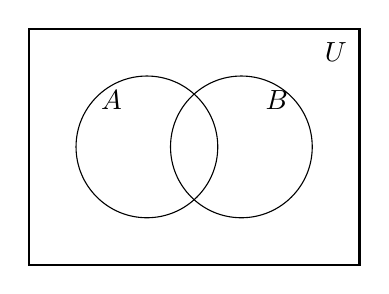
\begin{tikzpicture}[scale=.6]
    \draw[thick] (0,0) rectangle (7,5);
    \node at (6.5,4.5) {$U$};
    \draw (2.5,2.5) circle (1.5cm);
    \draw (4.5,2.5) circle (1.5cm);
    \node at (1.75,3.5) {$A$};
    \node at (5.25,3.5) {$B$};
\end{tikzpicture}
\end{exercise}

\begin{exercise}
Gegeven is dat $A$ de \textit{verzameling is van rode dingen}, en $B$ de \textit{verzameling van grote dingen}, en $x$ een variabele is over een universum $U$ (van objecten). Druk de volgende verzamelingen uit in $A$ en $B$ en de operatoren op verzamelingen:
\begin{enumerate}[label=\textit{\alph*.}]
    \item De verzameling $I$ van objecten die groot zijn als ze rood zijn.
    \item De verzameling $C$ van objecten die rood en groot zijn.
    \item De verzameling $E$ van objecten die rood zijn dan en slechts dan als ze groot zijn.
    \item De verzameling $D$ van objecten die rood of groot zijn.
\end{enumerate}
\end{exercise}

\begin{exercise}
Teken de bijbehorende Venn-diagrammen, en bewijs
\begin{enumerate}[label=\textit{\alph*.}]
    \item $A-(B-C)=A-(B-(A\cap C))$
    \item $(A-B)-C=A-(B\cup C)$
    \item $A-B=A-(A\cap B)$
    \item $A-B=(A\cup B)-B$
    \item $(A\Delta B)\cap C=(A\cap C)\Delta(B\cap C)$
\end{enumerate}
\end{exercise}

\begin{exercise}
Bestudeer de volgende uitspraken. Geef in geval van algemene juistheid een bewijs, geef anders een tegenvoorbeeld.
\begin{enumerate}[label=\textit{\alph*.}]
    \item $A-B=(A\cup C)-(B\cup C)$
    \item $A-B=(A\cap C)-(B\cap C)$
    \item $(A-B)\cup C=(A\cup C)-(B\cup C)$
    \item $(A-B)\cap C=(A\cap C)-(B\cap C)$
    \item $(A\Delta B)\cup C=(A\cup C)\Delta(B\cup C)$
\end{enumerate}
\end{exercise}

\begin{exercise}
Voor een verzameling $X$ met eindig veel elementen, geven we met $|X|$ het aantal elementen van $X$ aan. Alle in deze opgave voorkomende verzamelingen worden geacht eindig veel elementen te bezitten.
\begin{enumerate}[label=\textit{\alph*.}]
    \item Beredeneer dat $|A\cup B|=|A| + |B| - |A\cap B|$
    \item Gebruik het resultaat van a. om aan te tonen dat
    $$|(A\cup B\cup C)=|A|+|B|+|C|-|A\cap B|-|A\cap C|-|B\cap C|+|A\cap B\cap C|.$$
\end{enumerate}
\end{exercise}

\section{Machtsverzameling en cartesisch product}\label{sec:power}
Objecten hoeven geen ``ondeelbare'' dingen te zijn. Het komt zelfs vaak voor dat we hele verzamelingen als objecten wensen te beschouwen. Denk bijvoorbeeld aan een elftal, een regiment, een mierenkolonie.

Wellicht heb je op de middelbare school iets dergelijks ook gezien bij kansrekening, waar bijvoorbeeld gevraagd kan worden naar het aantal mogelijkheden waarop men uit een verzameling $V$ met $n$ objecten een groep kan maken. Dat is de vraag naar het aantal deelverzamelingen van $V$. Dat is het aantal \textit{elementen} van \emph{de verzameling bestaande uit de \textit{deelverzamelingen} van $V$}.

\newcommand{\power}{\ensuremath{\mathcal{P}}}

Deze verzameling noemen we de \textit{machtsverzameling} van $V$. In het Engels heet dit de \textit{power set}; we noteren hem dan ook met $\power(V)$:
$$\power(V) = \{A\;|\; A\subseteq V\}$$

We geven een voorbeeld. Zij $V=\{a,b,c\}$. Dan is 
$$\power(V)=\{\varnothing, \{a\},\{b\},\{c\},\{a,b\},\{a,c\},\{b,c\},\{a,b,c\} \}.$$

$\power(V)$ heeft in dit voorbeeld dus $8 (=2^3)$ elementen. In het algemeen bestaat $\power(V)$ uit $2^n$ elementen als $V$ uit $n$ elementen bestaat. Dit is als volgt in te zien. Een element van $\power(V)$ is een deelverzameling van $V$, en die ligt vast door voor elk element aan te geven of die wel of niet in de deelverzameling zit. Als $V$ bestaat uit $n$ elementen heb je hierbij dus $n$ keer een keuze uit twee mogelijkheden. In totaal levert dat $2^n$ mogelijkheden. Elke mogelijkheid correspondeert met precies \'e\'en deelverzameling, en elke deelverzameling kan zo worden verkregen, dus heeft $\power(V)$ precies $2^n$ elementen. Vanwege deze eigenschap wordt de machtsverzameling $\power(V)$ ook wel genoteerd als $2^V$; het woord \textit{machtsverzameling} is zo gekozen omdat hier sprake is van \textit{machtsverheffen}.

\begin{quote}
    Merk op dat we een onderscheid dienen te maken tussen het element $a$ en de verzameling $\{a\}$ die $a$ als enige element heeft.
    
    \noindent
    In het voorbeeld geldt wel $a\in \{a\}$ en $a\in V$ en $\{a\}\in\power(V)$ en $\{a\}\subseteq V$, maar niet $\{a\}\subseteq\power(V)$. Wel geldt $\{\{a\}\}\subseteq\power(V)$.
\end{quote}

Onder het \textit{cartesisch product} $A\times B$ van twee verzamelingen $A$ en $B$ verstaan we de verzameling van alle \textit{geordende paren} $(x,y)$ waarvoor $x\in A$ en $y\in B$.

Dat de paren geordende paren zijn, betekent dat $(x,y)$ en $(y,x)$ verschillend zijn als $x\not=y$.
$$A\times B=\{(x,y)\;|\; x\in A\wedge y\in B\}$$

Een voorbeeld: Zij
$$A=\{a,b,c,d\}\text{ en }B=\{a,d,f,e,g\}.$$
Dan is
$$\begin{array}{ccclllllc}
A\times B & = & \bigl\{ 
  & (a,a), & (a,d), & (a,f), & (a,e), & (a,g), & \\
  &&& (b,a), & (b,d), & (b,f), & (b,e), & (b,g), & \\
  &&& (c,a), & (c,d), & (c,f), & (c,e), & (c,g), & \\
  &&& (d,a), & (d,d), & (d,f), & (d,e), & (d,g), & \bigr\} \\
\end{array}$$

Als $A$ en $B$ eindige verzamelingen zijn met respectievelijk $n$ en $m$ elementen, heeft het cartesisch product $A\times B$ precies $n\times m$ elementen: voor elk geordend paar hebben we $n$ mogelijkheden om het eerste argument te kiezen en $m$ mogelijkheden om het tweede argument te kiezen. Dit verklaart waarom we dit een \textit{product} noemen. Het voorvoegsel is afgeleid van de wiskundige Ren\'e \textit{Descartes} (1596-1650), die de punten in het platte vlak opvatte als geordende paren van re\"ele getallen: de \textit{co\"ordinaten}.

Een reden dat we de begrippen machtsverzameling en cartesisch product als laatste hebben genoemd, is in de eerste plaats omdat ze abstracter (en wellicht onbekender) zijn dan de overige begrippen. Een andere reden is, dat deze constructies ons buiten een gegeven universum kunnen brengen. Men kan gemakkelijk zelf voorbeelden hiervan vinden.

\subsection{Opgaven}
\begin{exercise}\mbox{}
\begin{enumerate}[label=\textit{\alph*.}]
\item Gegeven is $A=\{1,2\}$ en $B=\{a,b\}$, bereken $A\times B$;
\item Gegeven is $A=\{1,2\}$ en $B=\{a,b\}$, bereken $B\times A$;
\item Gegeven is $Z=\{0,1,7,8\}$ en $Y=\{0,1\}$, bereken $Z\times Y$;
\item Gegeven is $A=\{f,k\}$ en $B=\varnothing$, bereken $A\times B$;
\item Gegeven is $V=\{f,t\}$ en $S=\{c,d,u\}$, bereken $V\times S$.
\end{enumerate}
\end{exercise}

\begin{exercise} Bereken:
\begin{enumerate}[label=\textit{\alph*.}]
\item $\power(A)$ als $A = \{1,3,4,5\}$;
\item $\power(B)$ als $B=\{\varnothing, 1,3\}$;
\item $\power(C)$ als $C=\{1,\{2,3\},\{\{4,5\}\}\}$.
\end{enumerate}
\end{exercise}

\begin{exercise}\mbox{}
\begin{enumerate}[label=\textit{\alph*.}]
\item Als $A$ een verzameling is en $|A|=5$, wat is dan $|\power(A)|$?
\item Als $A$ een verzameling is en $|A|=5$, wat is dan $|A\times A|$?
\item Als $A=\{12,14,5,1\}$, wat is dan $|(A\times A)\cup A|$?
\end{enumerate}
\end{exercise}

\begin{exercise} Bepaal voor elk van de volgenden of deze een power set zijn van een of andere verzameling $A$ (en definieer wat $A$ dan precies is). Neem aan dat $a$ en $b$ verschillende elementen zijn.
\begin{enumerate}[label=\textit{\alph*.}]
\item $\varnothing$;
\item $\{\varnothing,\{a\}\}$;
\item $\{\varnothing,\{a\},\{\varnothing,\{a\}\}\}$;
\item $\{\varnothing,\{a\},\{b\},\{a,b\}\}$.
\end{enumerate}
\end{exercise}

\begin{exercise}[Bonus]\mbox{}\\
Vindt twee verzamelingen $A$ en $B$ zodanig dat $A\in B$ \'en $A\subseteq B$.
\end{exercise}

\section{Functies}\label{sec:functies}
Wanneer we voor twee verzamelingen $A$ en $B$ bij elk element van $A$ precies \'e\'en element van $B$ vastleggen, dan hebben we een \textit{afbeelding} van $A$ naar $B$ gedefinieerd. In plaats van afbeelding zegt men ook wel \textit{functie}. In het Engels heet een afbeelding een \textit{map} of \textit{function}.

Door middel van een afbeelding van $A$ naar $B$ wijst elk element van $A$ dus een element van $B$ aan. Een element van $B$ kan vaker aangewezen worden. Een element van $A$ kan niet meer dan \'e\'en element van $B$ aanwijzen. Wij zullen ons meestal bedienen van deze terminologie van aanwijzen. Dit komt ook overeen met de veelgebruikte manier om een afbeelding van $A$ naar $B$ te visualiseren door middel van een tekening waarin vanuit elk punt van een getekende verzameling $A$ een pijl vertrekt die aankomt in een van de punten van de getekende verzameling $B$.
\begin{center}
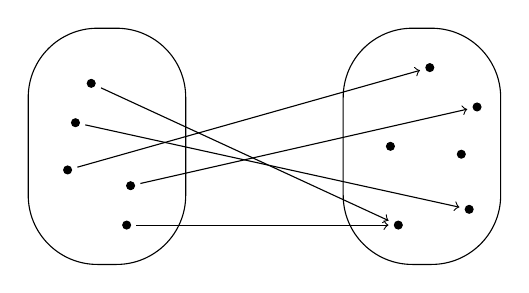
\begin{tikzpicture}
\draw[rounded corners=25pt] (0,0) rectangle (2,3);
\draw[rounded corners=25pt] (4,0) rectangle (6,3);
\draw[fill] (1.25, .5) circle (.05cm) node (a1) {};
\draw[fill] (1.3, 1) circle (.05cm) node (a2) {};
\draw[fill] (0.5, 1.2) circle (.05cm) node (a3) {};
\draw[fill] (0.6, 1.8) circle (.05cm) node (a4) {};
\draw[fill] (0.8, 2.3) circle (.05cm) node (a5) {};
\draw[fill] (4.7, .5) circle (.05cm) node (b1) {};
\draw[fill] (5.6, .7) circle (.05cm) node (b2) {};
\draw[fill] (4.6, 1.5) circle (.05cm) node (b3) {};
\draw[fill] (5.5, 1.4) circle (.05cm) node (b4) {};
\draw[fill] (5.7, 2.0) circle (.05cm) node (b5) {};
\draw[fill] (5.1, 2.5) circle (.05cm) node (b6) {};

\draw[->] (a1) -- (b1);
\draw[->] (a2) -- (b5);
\draw[->] (a3) -- (b6);
\draw[->] (a4) -- (b2);
\draw[->] (a5) -- (b1);
\end{tikzpicture}
\end{center}

Zo'n plaatje heet ook wel een \textit{pijlendiagram}.

Een afbeelding bestaat dus uit een drietal: een verzameling $A$, een verzameling $B$, en een beschrijving die aangeeft hoe de aanwijzing van elementen van $B$ door de elementen van $A$ er uitziet.

Korten we die beschrijving af door een letter, bijvoorbeeld $f$, dan is de afbeelding dus het drietal $(A, B, f)$.
$$A\text{ heet het \textit{domein} van }f\text{ (Engels: \textit{domain}),}$$
$$B\text{ heet het \textit{codomein} van }f\text{ (Engels: \textit{codomain}).}$$

Een suggestieve en zeer vaak gebruikte notatie is
$$f: A\rightarrow B.$$
Alhoewel de pijl hier verward zou kunnen worden met de logische pijl, staat de context er vrijwel altijd borg voor dat dit niet gebeurt. De combinatie $A\rightarrow B$ van domein en codomein heet wel het \textit{type} van de afbeelding $f$. Voor het codomein zul je soms ook de term \textit{bereik} (Engels: \textit{range}) tegenkomen; deze term wordt echter ook gebruikt voor een ander, gerelateerd, concept dat verderop besproken wordt, en zal in deze tekst verder vermeden worden.

Is $x$ een element van $A$, dan duidt $f(x)$ het \textit{beeld} van $x$ aan (Engels: \textit{image}), het element van $B$ dat door $x$ wordt aangewezen. Het element $x$ heeft dan wel het \textit{argument} van de afbeelding.

Twee afbeeldingen $f:A\rightarrow B$ en $g:C\rightarrow D$ zijn aan elkaar \textit{gelijk} (en dus dezelfde afbeelding), precies dan als aan drie voorwaarden voldaan is:
\begin{enumerate}
    \item $A = C$;
    \item $B = D$;
    \item voor alle $x\in A$ geldt dat $f(x) = g(x)$.
\end{enumerate}
\begin{example}
Enkele voorbeelden van afbeeldingen zijn:
\begin{itemize}
    \item $A=\mathbb{R}, B=\mathbb{R},$ voor alle $x\in\mathbb{R}$ is $f(x)=\text{sin}(x)$;
    \item $A=\{1, 2, 3\}, B=\{a, b, c, d\}, f(1)= b, f(2) = d, f(3) = b$;
    \item $A=\mathbb{N}, B=\{2,3,5,6\},$ voor alle $n\in\mathbb{N}$ is $f(n)=5$.
\end{itemize}
In het vervolg zullen we het tweede voorbeeld nog een aantal keren aanhalen. Enkele gevallen waarin we niet met een afbeelding van doen hebben, zijn:
\begin{itemize}
    \item $A=\mathbb{R}, B=\mathbb{R}, f(x)=\text{ln}(x)$,\\ want $\text{ln}(x)$ is niet voor elke $x\in\mathbb{R}$ gedefinieerd.
    \item $A=\mathbb{N}, B=\mathbb{Q}, f(x)=\sqrt{x}$,\\ want $\sqrt{2}\not\in\mathbb{Q}$.
\end{itemize}\label{vb:func}
\end{example}

Bij een afbeelding $f:A\rightarrow B$ en een deelverzameling $X$ van $A$ kunnen we kijken naar de deelverzameling van $B$ bestaande uit de beelden van alle elementen van $X$. Deze deelverzameling van $B$ heet het \textit{beeld} (Engels: \textit{image}) van $X$, en wordt aangeduid met $f(X)$. Ook het beeld wordt vaak aangeduid met de term \textit{bereik}; het kan dus per tekst verschillen of met deze term het grotere codomein bedoeld wordt, of de deelverzameling van het beeld. In deze tekst gebruiken we de ondubbelzinnige termen \textit{codomein} en \textit{bereik}, en raden jullie aan hetzelfde te doen.
$$f(X) = \{y\in B\;|\;\text{er is een } x\in X(y=f(x))\}$$
Merk op dat zowel de notatie als de terminologie hiervan overeenkomt met het beeld van een element. Uit de context moet dus worden opgemaakt om welk van de twee begrippen het gaat: als $x$ een element is van $A$ dan is $f(x)$ het bijbehorende element van $B$; als $x$ een deelverzameling is van $A$ dan is $f(x)$ de deelverzameling van $B$ bestaande uit bij die deelverzameling horende elementen van $B$.

In het voorbeeld van \ref{vb:func} hebben we onder andere
$$f(\{1\})=\{b\}, f(\{1,2\})=\{b,d\}, f(\{1,3\})=\{b\},f(A)=\{b,d\}$$

De verzameling $f(A)$ wordt wel het \textit{beeld} van $f$ genoemd. Ook kunnen we bij een deelverzameling $Y$ van $B$ vragen naar de deelverzameling van $A$ bestaande uit alle $x$ waarvoor $f(x)\in Y$.

In bijlage \ref{app:functies} wordt nog meer eigenschappen en bijzonderheden van functies besproken.

\subsection{Opgaven}

\begin{exercise}
  Ga na of de volgende relaties tevens functies zijn:\mbox{}\\
  \begin{enumerate}[label=\textbf{\alph*.}]
    \item de relatie kind-ouder;
    \item de relatie tussen een persoon en de verzameling van diens ouders;
    \item de relatie tussen een persoon en diens vaste partner;
    \item de relatie tussen een geheel getal en het getal met $1$ opgehoogd;
    \item de relatie tussen een getal en het kwadraat van dat getal;
    \item de relatie tussen een getal en de vierkantswortel van dat getal.
  \end{enumerate}
\end{exercise}

\begin{exercise}\mbox{}\\
  \begin{enumerate}[label=\textbf{\alph*.}]
    \item Gegeven zijn de verzamelingen $K = \{ \text{Wilhelmina}, \text{Juliana}, \text{Beatrix},$\\ $\text{Willem-Alexander}, \text{Amalia} \}$ en de volgende pijlen:
  \begin{align*}
    \text{Wilhelmina} &\longrightarrow \text{Juliana}\\
    \text{Juliana} &\longrightarrow \text{Beatrix}\\
    \text{Beatrix} &\longrightarrow \text{Willem-Alexander}\\
    \text{Willem-Alexander} &\longrightarrow \text{Amalia}
  \end{align*} Hebben we hier met een geldige functie $K \to K$ te maken?\\ Zo nee, wat zouden we moeten aanpassen om wel een geldige functie te defini\"{e}ren?\\

  \item Gegeven zijn de verzameling $H = \{ \text{steen}, \text{papier}, \text{schaar} \}$ en de volgende pijlen:
  \begin{align*}
    \text{steen} &\longrightarrow \text{schaar}\\
    \text{papier} &\longrightarrow \text{steen}\\
    \text{schaar} &\longrightarrow \text{papier}
  \end{align*} Hebben we hier met een geldige functie $H \to H$ te maken?\\ Zo nee, wat zouden we moeten aanpassen om wel een geldige functie te defini\"{e}ren?
  \end{enumerate}
\end{exercise}

\begin{exercise}\mbox{}\\
  \begin{enumerate}[label=\textbf{\alph*.}]
    \item Gegeven zijn de verzameling $S = \{ \text{winter}, \text{lente}, \text{zomer}, \text{herfst} \}$ en de afbeelding $v : S \to S$:
  \begin{equation*}
  \begin{aligned}
    \text{winter} &\longrightarrow \text{lente}\quad\quad\quad &
    \text{zomer} &\longrightarrow \text{herfst}\\
    \text{lente} &\longrightarrow \text{zomer}&
    \text{herfst} &\longrightarrow \text{winter}
  \end{aligned}
  \end{equation*}
  \begin{enumerate}[label=\textbf{\alph*.}]
      \item Wat is de waarde van $v(\text{zomer})$?
      \item Wat is het type\footnote{Tot welke verzameling behoort deze waarde?} van $v(\text{zomer})$?
      \item Heeft het zin om over de waarde $v(v(\text{winter}))$ te redeneren?\\ Zo ja: wat is deze waarde; zo nee: waarom niet?\\
  \end{enumerate}

  \item Gegeven zijn de verzamelingen $D_{1} = \{ \text{David}, \text{Matt}, \text{Peter} \}$, $D_{2} = \{ \text{Matt}, \text{Peter}, \text{Jodie} \}$ en de afbeelding $r : D_{1} \to D_{2}$:
  \begin{equation*}
  \begin{aligned}
    \text{David} &\longrightarrow \text{Matt}\quad\quad
    \text{Peter} &\longrightarrow \text{Jodie}\\
    \text{Matt} &\longrightarrow \text{Peter}
  \end{aligned}
  \end{equation*}
  \begin{enumerate}[label=\textbf{\alph*.}]
      \item Wat is de waarde van $r(\text{David})$?
      \item Wat is het type van $r(\text{David})$?
      \item Heeft het zin om voor $x \in D_{1}$ over de waarde $r(r(x))$ te redeneren?\\ Beargumenteer je antwoord.
  \end{enumerate}
  \end{enumerate}
\end{exercise}

\begin{exercise}\mbox{}\\
  \begin{enumerate}[label=\textbf{\alph*.}]
    \item Gegeven is de functie $f(x) = 2x + 1$. We kunnen hier verschillende keuzes voor het domein maken; het codomein zal hiervan afhankelijk zijn.
      \begin{enumerate}
        \item Wat is het codomein als het domein $\mathbb{N}$ is?
        \item Wat is het beeld\footnote{Hint: voor deze verzameling hebben we geen symbool zoals $\mathbb{N}$, maar toch is deze eenduidig te beschrijven als deelverzameling van het codomein dat je al gevonden hebt.} als het domein $\mathbb{N}$ is?
        \item Wat is het codomein als het domein $\mathbb{R}$ is?
      \end{enumerate}

    \item Gegeven is de functie $f(x) = 3^{x} - 2$. We kunnen hier verschillende keuzes voor het domein maken; het codomein zal hiervan afhankelijk zijn.
      \begin{enumerate}
        \item Wat is het codomein als het domein $\mathbb{N}$ is?
        \item Wat is het codomein als het domein $\mathbb{N}_{1}$ is, waarbij $\mathbb{N}_{1} = \mathbb{N} - \{0\}$, oftewel de verzameling van alle positieve gehele getallen?
        \item Wat is het codomein als het domein $\mathbb{Z}$ is?
        \item Wat is het codomein als het domein $\mathbb{Q}$ is?
      \end{enumerate}


  \end{enumerate}
\end{exercise}
